%---------------------导言区---------------------------%
\documentclass[12pt,a4paper,UTF8]{ctexart}
	%10pt:正文字体为12pt,缺省为10pt;各层级字体大小会根据正文字体自动调整
	%a4paper:纸张大小a4;
	%UTF8:中文要求
%\usepackage{syntonly}
%\syntaxonly%加快编译速度
\usepackage{geometry}%用于设置上下左右页边距
	\geometry{left=2.5cm,right=2.5cm,top=3.2cm,bottom=2.8cm}
\usepackage{xeCJK,amsmath,paralist,enumerate,booktabs,multirow,graphicx,float,subfig,setspace,listings,lastpage,hyperref,gensymb}
	%xeCJK:中文字体(如楷体,作者和机构需要用到)的设置
	%amsmath:数学公式
	%paralist,enumerate:自定义项目符号
	%booktabs:三线图,论文常用的表格风格
	%multirow:复杂表格
	%graphicx,float: 插入图片
	%subfig:并排排版图片以及强制图表显示在“这里”[H]
	%setspace:设置行间距等功能
	\setlength{\parindent}{2em}%正文首行缩进两个汉字
	%listings:用于排版各种代码;比如matlab的代码
	%\lstset{language=Matlab}%matlab代码
	%lastpage:获取总页数;
	%hyperref:超链接,和lastpage搭配.
\usepackage{pifont}
\usepackage{fancyhdr}
	%fancyhdr:一个很强大的宏包,用于自定义设计页面风格并命名以供调用。
	\pagestyle{fancy}
	\rhead{实验十七~$RLC$电路的谐振现象}
	\lhead{普通物理实验\uppercase\expandafter{\romannumeral1}实验报告}
	\cfoot{\thepage}  
		%分别是右页眉、左页眉、右页脚
	\renewcommand{\headrulewidth}{0.4pt}
	\renewcommand{\theenumi}{(\arabic{enumi})}

\setCJKmainfont{FZSSK.TTF}[ItalicFont=FZKTK.TTF, BoldFont=FZHTK.TTF]
%中文字体设置:使用开源字体方正书宋,方正楷体和方正黑体



%%%%%%%%%%%%%%%%%%%%%%%%%%%%%%%%%%%%%%%%%%%%%%%%%%%%%%%%%%
%%%%%%%%%%%%%%%%%%%%%%%%%正文开始%%%%%%%%%%%%%%%%%%%%%%%%%%
%%%%%%%%%%%%%%%%%%%%%%%%%%%%%%%%%%%%%%%%%%%%%%%%%%%%%%%%%%

\begin{document}

%%begin-------------------标题与信息-----------------------%%

%%标题
\begin{center}
\LARGE\textbf{实验十七~$RLC$电路的谐振现象}
\end{center}

%%信息
\begin{doublespacing}
	%doublespacing:手动两倍行距
	\centering
	\begin{tabular}{ll}
	 & \\
	{\CJKfontspec{STKAITI.TTF} 实验人:钟易轩}  & {\CJKfontspec{STKAITI.TTF}指导教师:彭莹莹}\\
	{\CJKfontspec{STKAITI.TTF} 组号:九组七号} & {\CJKfontspec{STKAITI.TTF}学号:2000012706}\\
	{\CJKfontspec{STKAITI.TTF} 实验时间:2021年12月17日} &{\CJKfontspec{STKAITI.TTF} 实验地点:物理楼南楼~234}
	\end{tabular}
\end{doublespacing}

%%end-------------------标题与信息-----------------------%%

\subsection*{【实验目的】}
	\begin{enumerate}[(1)]
		\item 研究$RLC$电路的谐振现象;
		\item 了解$RLC$电路的相频特性和幅频特性;
	\end{enumerate}
	
\subsection*{【数据处理】}
\subsubsection*{1.谐振状态下的测量结果}
将示波器调整为“x-y”模式,调节信号发生器的频率,当示波器中曲线由椭圆变为直线时,说明达到谐振状态,此时$f_0=2.251(\mathrm{kHz})$.在此状态下,数据如表1所示.
\begin{table}[htbp]
\centering
\caption{谐振状态下的测量结果}
\scalebox{1.1}{
\begin{tabular}{cccccc}
\toprule
$U_{\text{总} 1}/\rm{V}$&$U_R/\rm{V}$&$U_{\text{总} 2}/\rm{V}$&$U_C/\rm{V}$&$C/\rm{\mu F}$&$L/\rm{H}$ \\
\hline
2.840&2.195&1.0001&10.789&0.05&0.1 \\
\bottomrule
\end{tabular}}
\end{table}\par
对于$Q_1=\dfrac{1}{\omega_0R_{\text{总}}C}$来说,$R_{\text{总}}$并不好测,因此采用$R_{\text{总}}=\dfrac{U_{\text{总}}}{U_R}R$来间接计算$R_{\text{总}}$.
\begin{align*}
	R_{\text{总}}&=\frac{2.840}{2.195}\times100=129.38(\Omega) \\
	\omega_0&=2\pi f_0 \\
	Q_1&=\frac{1}{\omega_0R_{\text{总}}C}=10.93 \\
	Q_2&=\frac{U_C}{U_{\text{总}}}=10.79 \\
\end{align*}
\par
对$Q_1$与$Q_2$进行误差分析:\par
仪器的允差为$e_L=0.1\times0.1\%=0.0001(\rm{H})$,$e_C=0.05\rm{\mu F}\times0.65\%=0.325(\rm{nF})$,$\sigma_{f_0}=0.001\times10^3\div\sqrt{3}=0.6(\rm{Hz})$,$\sigma_{R_{\text{总}}}=0.07(\Omega)$.\par
则有
\begin{align*}
	\sigma_{Q_1}&=\sqrt{(\frac{\partial Q_1}{\partial \omega_0}\sigma_{\omega_0})^2+(\frac{\partial Q_1}{\partial R_{\text{总}}}\sigma_{R_{\text{总}}})^2+(\frac{\partial Q_1}{\partial C}\sigma_C)^2} \\
	&\approx0.07 \\
	\sigma_{Q_2}&=\sqrt{(\frac{\partial Q_2}{\partial U_C}\sigma_{U_C})^2+(\frac{\partial Q_2}{\partial U_{\text{总}}}\sigma_{U_{\text{总}}})^2} \\
	&\approx0.02 \\
\end{align*}
\par
因此,$Q_1=10.93\pm0.07$,$Q_2=10.79\pm0.02$.
\subsubsection*{2.相频特性数据表}
在测试相频特性时,有
\begin{align*}
	\Delta \varphi&=\varphi_U-\varphi_I \\
	&=\Delta t\times f\times 360^{\circ}
\end{align*}
\par
根据上式,可得表2.
\begin{table}[htbp]
\centering
\caption{相频特性数据表}
\scalebox{1.1}{
\begin{tabular}{lccccccc}
\toprule
$f/\mathrm{kHz}$&1.850&1.973&2.073&2.153&2.195&2.224&2.251 \\
\hline
$\Delta t/\mathrm{ms}$&-0.119&-0.102&-0.082&-0.057&-0.039&-0.021&0.002 \\
\hline
$\Delta \varphi/\circ$&-79.3&-72.4&-61.2&-44.2&-30.8&-16.8&1.6 \\
\hline\hline
$f/\mathrm{kHz}$&2.278&2.311&2.356&2.436&2.588&2.900& \\
\hline
$\Delta t/\mathrm{ms}$&0.017&0.037&0.055&0.068&0.079&0.075& \\
\hline
$\Delta \varphi/\circ$&13.9&30.8&46.6&59.6&73.6&78.3& \\
\bottomrule
\end{tabular}}
\end{table}\par
根据表2中数据,可以作出相频特性图.
\newpage
\begin{figure}[htbp]
		\centering
		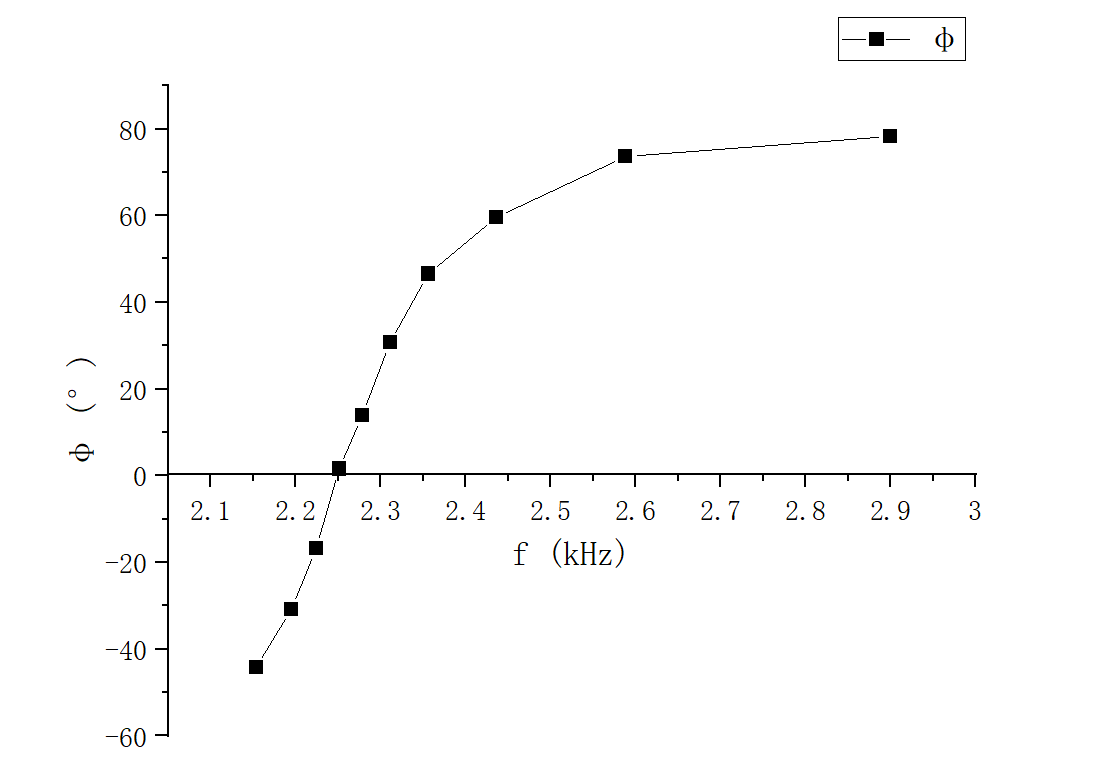
\includegraphics[width=9cm]{1.png}
		\caption{相频特性曲线图}
\end{figure}
\subsubsection*{3.幅频特性数据表}
\begin{table}[htbp]
\centering
\caption{幅频特性数据表}
\scalebox{1.1}{
\begin{tabular}{lcccccc}
\toprule
$f/\mathrm{kHz}$&1.850&1.900&1.973&2.000&2.073&2.100 \\
\hline
$U_R/mV$&174.9&200.8&253.7&279.5&377.3&428.1 \\
\hline\hline
$f/\mathrm{kHz}$&2.153&2.175&2.195&2.210&2.224&2.230 \\
\hline
$U_R/mV$&586.1&623.2&684.6&722.3&750.9&759.5 \\
\hline\hline
$f/\mathrm{kHz}$&2.251&2.260&2.278&2.300&2.311&2.320 \\
\hline
$U_R/mV$&774.6&769.8&745.8&696.1&665.6&641.0 \\
\hline\hline
$f/\mathrm{kHz}$&2.356&2.400&2.436&2.500&2.588&2.700 \\
\hline
$U_R/mV$&543.2&445.4&384.5&306.4&238.6&186.5 \\
\hline\hline
$f/\mathrm{kHz}$&2.900&2.149&2.354& & &  \\
\hline
$U_R/mV$&135.3&547.7&547.7& & & \\
\bottomrule
\end{tabular}}
\end{table}
\par
若要转化为电流,那么只需将表3中的$U_R$除以100即可.根据上表中原始数据转换得到的电流数据可以作出如下图像.
\newpage
\begin{figure}[htbp]
		\centering
		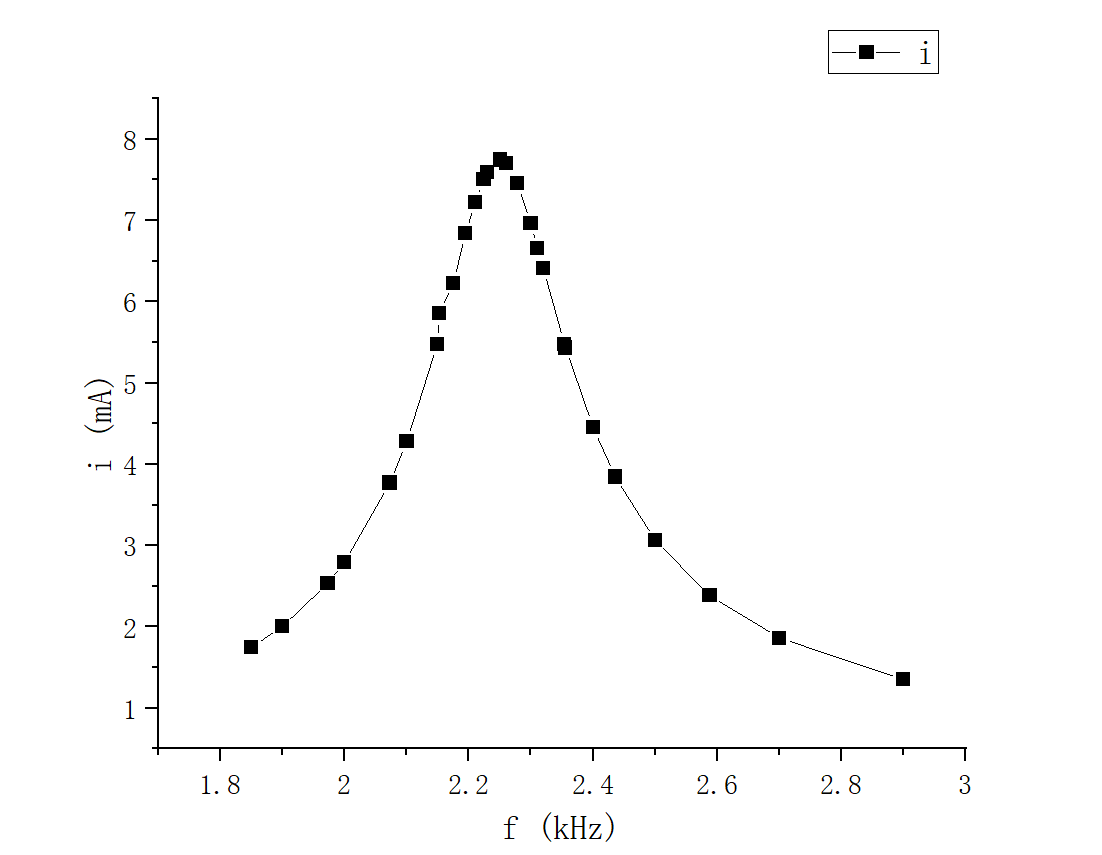
\includegraphics[width=9cm]{3.png}
		\caption{幅频特性曲线图}
\end{figure}
\par
可以算得$Q_3=\dfrac{f_0}{\Delta f}=\dfrac{2.251}{2.354-2.149}=10.98$.且有
\begin{align*}
	\sigma_{Q_3}&=\sqrt{(\frac{\partial Q_3}{\partial f_0}\sigma_{f_0})^2+(\frac{\partial Q_3}{\partial \Delta f}\sigma_{\Delta f})^2} \\
	&=0.03
\end{align*}
\par
则有$Q_3=10.98\pm0.03$.
\subsubsection*{4.黑盒子实验}
选取的是7号黑盒子,当$f=3.085\rm{kHz}$时达到谐振状态,因此应该是电容电感电阻串联.在谐振状态下,$\omega L-1/\omega C=0$,则有$|Z|=R=177.03\div707.2\times100=25.05(\Omega)$.又测试了两个状态,如表4所示.
\begin{table}[htbp]
\centering
\caption{黑盒子数据表}
\scalebox{1.1}{
\begin{tabular}{ccc}
\toprule
$f/\rm{kHz}$&$U_R/\rm{mV}$&$U_i/\rm{mV}$ \\
\hline
3.096&706.3&177.3 \\
\hline
3.146&702.4&184.3 \\
\bottomrule
\end{tabular}}
\end{table}
\par
根据上表可联立方程解出$C=267.68(\rm{nF})$,$L=9.957(\rm{mH})$.
\subsection*{【思考题】}
(1)对谐振频率$f_0$来说,有
\begin{equation*}
	f_0=\frac{1}{2\pi\sqrt{LC}} \tag{17.1}
\end{equation*}
说明$f_0$与R无关,故谐振频率不会变化.而对于其他参量,则有
\begin{align*}
|Z|&=\sqrt{R^2+(\omega L-1/\omega C)^2} \\
\tan\varphi&=\frac{\omega L-1/\omega C}{R} \\
i&=\frac{u}{\sqrt{R^2+(\omega L-1/\omega C)^2}} \\
Q&=\frac{\omega_0L}{R}=\frac{1}{R\omega_0C}
\end{align*}
因此,电流会变小,阻抗会增大,且品质因数$Q^{\prime}=0.2Q$,$\tan\varphi^{\prime}=0.2\tan\varphi$.\par
(2)\ding{172}对于品质因数Q来说,还有另一种表示方法,即
\begin{equation*}
	Q=\frac{U_C}{U} \tag{17.2}
\end{equation*}
因此可以依靠仪器中的电压表测出的数据计算出Q值.\par
\ding{173}将信号源频率调至谐振频率,测出此时的$U_C$与$U$,利用上述公式计算出Q.\par
\ding{174}先计算Q值:
\begin{equation*}
	Q=\frac{u_C}{u}=\frac{1000}{10}=100
\end{equation*}
由(17.1)式得,已知$C$与$f_0$的情况下,有$L=2.13\times10^{-4}(\rm{H})$.又根据$Q=\dfrac{\omega_0L}{R_r}$得,
\begin{equation}
	R_r=\frac{2\pi f_0L}{Q} \tag{17.3}
\end{equation}
则有$R_r=8.03(\Omega)$.
\subsection*{【分析与讨论】}
1.实验中测得的曲线都以$f_0$为转折点,阻抗特性图与幅频特性图是以$f_0$为一阶导数的转折点,而相频特性图则是以$f_0$为二阶导数的转折点.\par
2.根据计算结果表明,$\sigma_{Q_2}$是最小的,$\sigma_{Q_1}$是最大的.且$Q_1$与$Q_3$更为接近,$Q_2$偏小.




\end{document}